\documentclass{sig-alternate}
\usepackage{url}

\title{FriendlyLocation: Using Tie Strength to Geo-locate Users
}
\numberofauthors{1} 
\author{
    \alignauthor Jeffrey McGee, James Caverlee\\
    \affaddr{Department of Computer Science and Engineering, Texas A\&M
    University} \\
    \affaddr{ College Station, TX 77845 USA} \\
    \email{jeffamcgee@tamu.edu, caverlee@cse.tamu.edu}
} 
\begin{document}

\maketitle
\begin{abstract}
With the rise of volunteered user location information through services like
Foursquare, Google Latitude, and Facebook Places, we face unprecedented access
to the trails and connections among millions of social media users. This
location information is increasingly being incorporated in social media for
providing localized content, location-aware recommendations, and other
geo-spatial enabled services. In this paper, we investigate the interplay of
distance and tie strength through an examination of 20 million geo-encoded
tweets collected from Twitter and 6 million user profiles. Concretely, we
investigate the relationship between the strength of the tie between a pair of
users, and the distance between the pair. We identify several factors --
including following, mentioning, and actively engaging in conversations with
another user -- that can strongly reveal the distance between a pair of users.
We find a bimodal distribution in Twitter, with one peak around 10 miles from
people who live nearby, and another peak around 2500 miles, further validating
Twitter's use as both a social network (with geographically nearby friends) and
as a news distribution network (with very distant relationships). Based on
these findings, we propose and evaluate a method for predicting location for
users based purely on an analysis of the user's social network, which has great
significance for augmenting traditional social media and enriching
location-based services with more refined and accurate location estimates.

\end{abstract}




\section{Introduction}

put things in context

Publicly available data
@mention
efficient


Discuss bimodal distribution.
talk about sections in document

\begin{figure}
\centering
\epsfig{file=edge_types_norm.pdf, width=\linewidth}
\caption{
Smoothed histogram of distance to users for different types of relationships.
The dotted black line was created by calculating the distance between random, unrelated users.
}
\label{fig:EdgeTypes}
\end{figure}


\section{Related Work}
\cite{scellato2011socio}
\cite{scellato2010distance}
\cite{backstrom2010find}
\cite{cheng2010you}
\cite{backstrom2008spatial}
\cite{gilbert2009predicting}
\cite{cranshaw2010bridging}
\cite{java2007we}
The triad paper?
Gilbert ?


\section{Data Collection}
We collected 

social networking and bloging sites.

We define the set of the user's friends, followers, and the users who they mention to be their contacts.
Twitter does not provide a mechanism to determine who mentioned a given user, and as a result, we do not consider these users to be contacts.
In some blogging platforms, such as Tumblr, it is relatively easy to find the communication edges that point back toward a user.
In those platforms, it would be fairly straightforward to use that information in location prediction.

Any given contact can be categorized into precisely one of these four disjoint sets:
\begin{description}
\item[reciprocal friend] The geo-located user follows this user and is followed back.
\item[just friend] The geo-located user follows this user and is not followed back.
\item[just follower]The geo-located user is followed by this user, but does not follow them.
\item[just mentioned] The users do not follow each other, but the geo-located user mentioned the name of the other user in a tweet.
\end{description}

We used Twitter's Streaming API to obtain 19877804 tweets that contain
geographic information and were posted between April 7 until April 16,2011.
We ignored tweets from users who made their account private, had neither
friends nor followers, or posted fewer than two tweets in the sample.
We found the median latitude and median longitude for each user, and use this
as an approximation of the home location of the user.
We noticed that some Twitter accounts, such as accounts that posted jobs, would
move around faster than a human could possibly move. To account for this, we
calculated the distance between each tweet and the user's home location. We
ignored users if the median distance from their tweets to their home location
was greater than 50 miles.

We considered users to be in the US based on a simple bounding box.  If their median latitude was between 24 and 50 degrees and their median longitude was between -126 and -66 degrees, then their home location was considered inside the continental US.
We divided these geo-located users into groups based on the last digit of their twitter user id:
\begin{description}
\item[0--6] The training group had 104214 users with a home location in the US bounding box. Some of these users were also used to evaluate the quality of geocoding. For geocoding, we chose users from around the world with a decodable location field and split them into two groups:
\begin{description}
\item[0--3] The geocoding training group has 131295 users.
\item[4--6] The geocoding evaluation group has 85664 users.
\end{description}
\item[7--9] The evaluation group had 40861 users with a home location in the US.
\end{description}

For all of the geo-located users who lived in the US, we used Twitter's API to download the users' friends, followers, and 100 most recent tweets.
We also downloaded the profiles for up to 2000 friends, followers, and people they mention in their tweets. If they had over 2000, we chose a random sample of 2000 profiles that included at least 25 of each of the four categories listed below.
From the profiles, we kept the users with a decodable location field and threw away the rest. From what was left, we randomly picked one Friend, one Follower, one Just Mentioned, and up to seven reciprocal friends.
For each of these contacts, we stored their friends, followers, and 100 most recent tweets.

\subsection{Geocoding}
We used Gisgraphy\footnote{\url{http://www.gisgraphy.com/}} to do geocoding.
Gisgraphy does full-text search on the GeoNames\footnote{\url{http://www.geonames.org/}}
database using Lucene. Since
it runs locally we are not limited to a certain number of queries per day.
Gisgraphy's geocoder returns ranked results based on a full text search
over millions of geographical features such as countries, cities, and schools. 

The location field on a user's profile is just a text field that asks the user to respond to "Where in the world are you?".
Responses vary from precise latitude and longitude coordinates entered automatically by smart phone apps to jokes and nonsense.
We had to do some preproccessing before sending user-submitted locations to the geocoder.
First, we used a regular expression to find latitude and longitude coordinates. These are treated as if they were a unique type of location returned by the geocoder.
Occasionally, users would put two locations separated by a slash, dash or a conjunction. If the geocoder did not return any results for a user, we tried to geocode both locations and used the first location that the geocoder understood.

We noticed that some locations are significantly more useful than others.
For example, even though Rhode Island and Montana are both states with around
one million people, Rhode Island is smaller, and as a result, much more useful
in estimating the location of a user.
To make the results of the geocoder more useful, we devised a method to estimate the accuracy of a location returned by the geocoder.
For the users in the geocoding training and evaluation groups, we have both the
home location based on geo-located tweets, and the free-response location field
that we did geocoding on.
Originally, we planned to just use the users in the US, but we found that users
in the US had friends outside of the US, so we need to estimate the quality of
locations outside of the US as well.
As a result, we trained on geographic data from around the world.

\begin{table}
\centering
\caption{Example Median Location Errors}
\begin{tabular}{l r r} 
Location&Number of Users&Median Error in Miles\\ \hline
``Bronx''&53&4\\
``New York''&1264&174\\
``Pluto''\footnote{According to Gisgraphy, Pluto is a city in the Philippines and not a planet.}&11&7843\\ \hline
\\
Place Type&Number of Users&Median Error in Miles\\ \hline
A Coordinate&25216&3\\
A City&7128&6\\
An Airport&117&31\\
A Country&37&3935\\
\hline\end{tabular}
\label{tab:MedianLocErr}
\end{table}

\begin{figure}
\centering
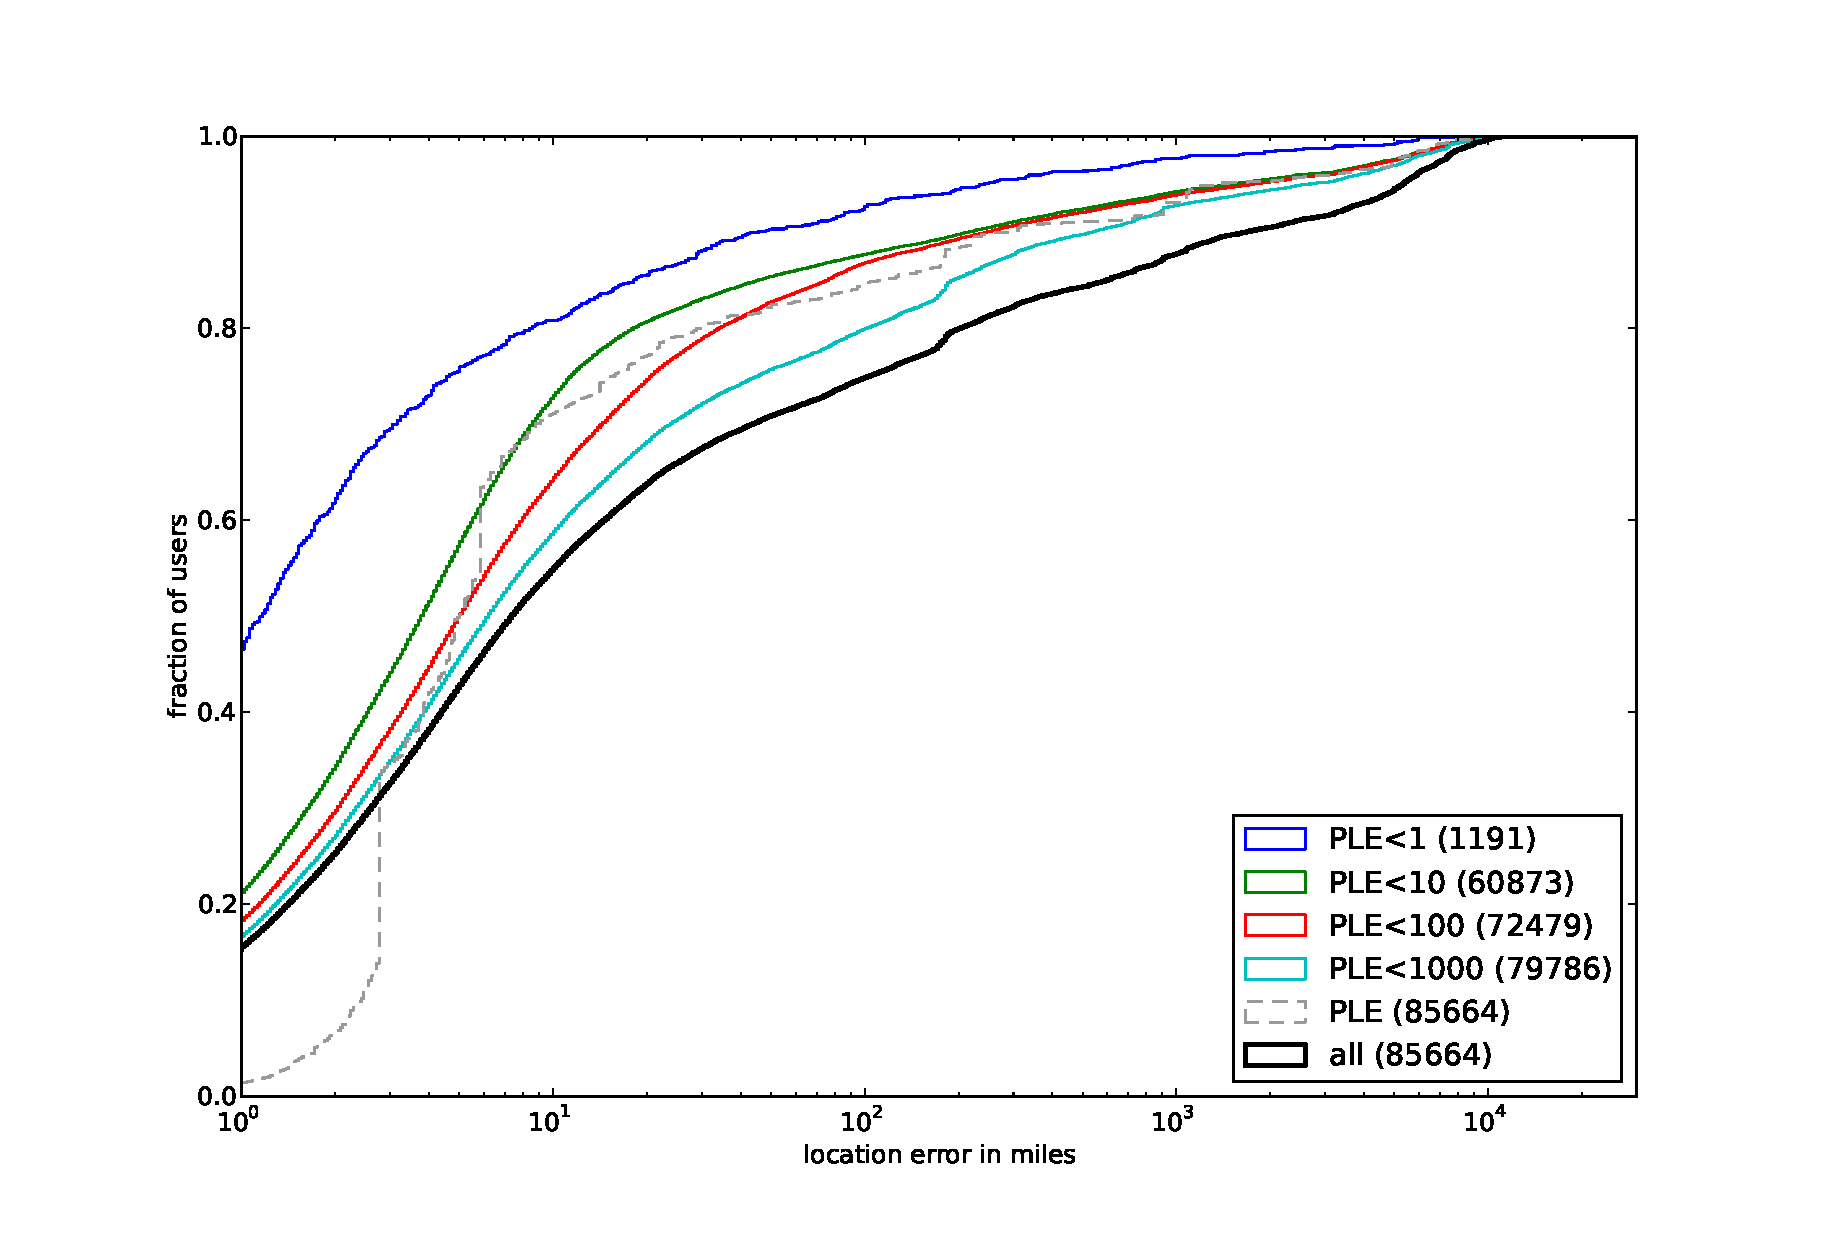
\epsfig{file=diff_gnp_gps.pdf, width=\linewidth}
\caption{
The dashed line shows the cumulative distribution function(CDF) of the predicted location error.
The other lines show the CDF of the actual location error for the geocoding evaluation group. The colored lines show how the location prediction improves when we remove users with a high PLE. For example, all the users in the "PLE<1" category have a predicted location error(PLE) of less than one mile.
In the legend, the number in parenthesis is the number of users in that category.
}
\label{fig:DiffGnpGps}
\end{figure}


\textsc{HAVERSINE!}

We define the location error to be the distance between a user's home location and the result from the geocoder.
The location error can vary from less than a mile to over ten thousand miles.
We ran the geocoder on each user in the geocoding training group, and then grouped users based on the result of the geocoder.
For the 3866 locations that had at least three users, we calculated the median location error for that location.
Next, we grouped all of the locations that had the same type and had one or two users, and calculated the median error for the location type.
We choose the median over average or standard deviation because those metrics are strongly affected by large outliers.
We choose to make the cutoff three because that is the smallest value where the median is not just an average.
Table \ref{tab:MedianLocErr} shows the median location error for a few example locations and location types.

We now have a method to predict the quality of a coordinate returned by Gisgraphy.
We define the predicted location error(PLE) for a given location to be median location error if it is one of the 3866 locations that had three users; otherwise, it is the median location error for the location's type.
For example one user had "PDX,OR" in his location field. Gisgraphy identifies this as "Portland International Airport". Since it is not one of the most common locations, its PLE is determined by its place type to be 31 miles as seen in Table \ref{tab:MedianLocErr}.

In Figure \ref{fig:DiffGnpGps}, we show the result of using the PLE to ignore users who have low quality locations such as "Pluto".
The solid black line represents the normal results of geocoding where the location error is less than 1000 miles for 88\% of the users.
The cyan line represents what happens when we remove locations with a PLE greater than or equal to 1000 miles. Now, after removing only 6\% of the users, 93\% of them are within 1000 miles.

\section{Investigation}
Every user who has multiple contacts will have some people who are much
closer than others. In order to estimate the locations of users, we would like
to find out which users are most likely to live nearby.  In this section, we
investigate how various types of contacts correlate with proximity.
All of the analysis in this section was done on the 104214 users with a home
location inside the US bounding box. We used their friends, followers, and the
people they mention with a PLE of less than 1000 miles.

\subsection{What type of contact is closest?}
\begin{figure}
\centering
\epsfig{file=edge_types_cuml.pdf, width=\linewidth}
\caption{
CDF of distance from geo-located users to users they have some contact
with.
The curves in this figure are the integrals of the curve in Figure \ref{fig:EdgeTypes}.
\textsc{Do we need this figure?}
}
\label{fig:EdgeTypesCum}
\end{figure}
In Figure \ref{fig:EdgeTypesCum} we look at the cumulative distribution
function(CDF) of the distance between a geo-located user and several types of
contacts.
Distance is plotted on a logarithmic scale to show both local and
global effects.

In general, reciprocal friends are the closest, followed by followers, friends,
and finally users who are just mentioned.
34\% of reciprocal friends live within 25 miles while only 18\% of users who are
just mentioned live within that radius.
While it may seem that since being followed by someone and following someone
should be identical, they are not.
Famous users on Twitter often have large numbers of followers, but they do not
follow a large number of users back.
Since the geo-located user was selected randomly, they are usually an average
user and not a celebrity.
If they follow someone, it might be a celebrity; however, if someone follows
them, it is probably someone who knows them.

There is a strange corner in the top right corner of all the graphs at
approximately 2500-2750 miles. This is caused by the large population living on the
coast, and the minuscule number of people posting tweets from the Atlantic and
pacific oceans.

\subsection{What is the distribution of contacts?}
To understand the distribution of, we created a smoothed histogram 
First, we sorted the distances into 200 logarithmically scaled bins (40 bins for each power of 10). Next, we convolved it with a seven element triangular window to smooth out the curve.
We used this procedure to plot each of the curves in Figure \ref{fig:EdgeTypes}.

All four types of contacts follow roughly the same bimodal distribution:
one peak around 10 miles from people who live nearby, and another peak around
2750 miles.

We shuffled the geo-located users and their reciprocal friends so that they
would be paired with someone who was probably not their friend and then
calculated the distance between the pair.
The dotted black line
shows the results of this procedure. For distances greater than around five
hundred miles, the red line and the black line have roughly the same shape,
which suggests that people when people are far away, their physical location no
longer matters.
The random line also has a similar shape to the other curves for distances
greater than 100 miles.

One reasonable explanation for this is that Twitter is not just a social
network; it is also an news distribution network.  This bimodal distribution
suggests that users have two types of contacts: people who they met in
real life, and people who they met online or know about via mainstream media.
The former group is useful for predicting location and the latter group is not.
In section \ref{sec:model}, we use this idea that there are two types of
contacts to build our model.

\subsection{Are users closer to people they communicate with?}
\begin{figure*}
\centering
\epsfig{file=com_types.pdf, width=\linewidth}
\caption{
CDF of the distance between a geo-located user and various types of contacts piloted on a logarithmic scale.
In these graphs, "I" refers to the geo-located user. "You" refers to their contact. 
}
\label{fig:ComTypes}
\end{figure*}
In Figure \ref{fig:ComTypes}, we investigate the relationship between various 
types of communication patterns.
Each of the four graphs visualize the same number of edges on the social graph with the exception of the Just Mentioned graph. Approximately one-third of our geo-located users never mentioned someone who was not a friend or a follower.

In almost every case, increased communication increases the probability that two users live near each other. There is one exception: when an average user mentions someone they follow who does not follow them back, it has no effect.
In other words, if a random user mentions a celebrity who does not bother to reply, they probably do not live in the same area. This can be seen by the blue and green lines that are right on top of each other in the Just Friend graph.
On the other hand, in the rare event that someone who is just a friend replies
to their follower, then the probability that they live near each other is much higher.

The weakest type of contact for users who are just mentioned, but never replied to, but if the person is mentioned, then 31\% of users with no friend/follow relationship who have a conversation live within 25 miles.
31\% of reciprocal friends who ignore each other live within 25 miles.
Unsurprisingly, the strongest type of connection is reciprocal friends who communicate.

\subsection{Are users closer to private accounts?}
\begin{figure}
\centering
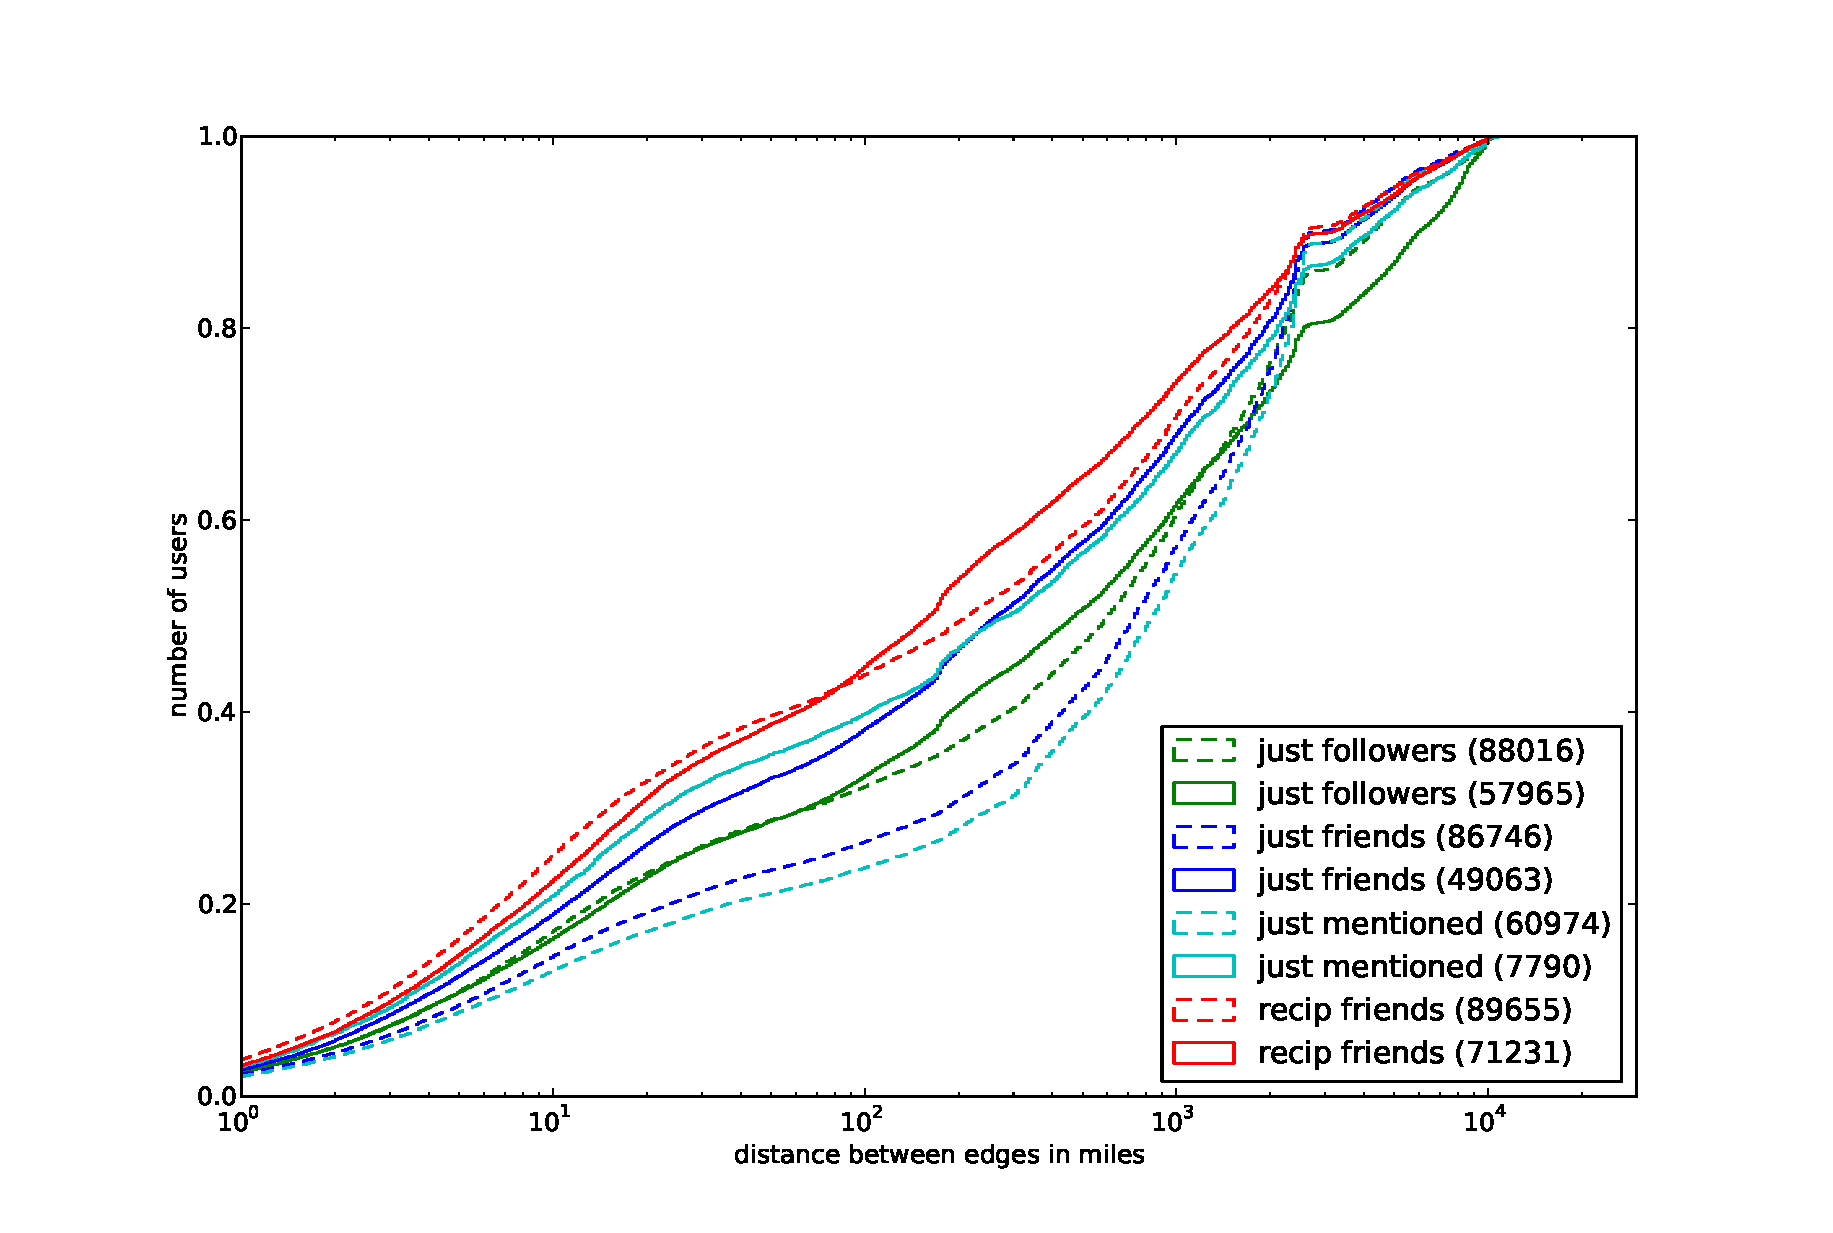
\epsfig{file=edge_types_prot.pdf, width=\linewidth}
\caption{Solid lines represent protected accounts, and dashed lines represent public accounts. If a user follows a protected account, they tend to be closer.}
\label{fig:EdgeTypesProt}
\end{figure}

Like many social networks, Twitter allows users to mark their account as protected. The specifics differ from network to network, but in Twitter's case a user has to be approved to follow a protected user.
In most of this section we are only concerned with public accounts, but in this subsection, we investigate how protected accounts compare to public accounts.
In the case of protected accounts on Twitter, we can download basic information
about their profile such as their location and the number of friends and
followers, but we cannot get their friends list, followers list, or the text of their tweets.

The most dramatic difference between private and public occurs if a user follows a protected account.
Since users generally only allow people they know to follow a protected account, this brings the users almost as close together as if they were reciprocal friends. On the other hand, if a protected account follows the geo-located user, this is almost insignificant.

\textsc{One possible explanation for the red lines crisscrossing is that a
protected account is more likely to live in a rural, unpopulated area. cite
Gilbert}

\subsection{If two of your friends live near each other, does that increase the chance that they live near you?}
\begin{figure}
\centering
\epsfig{file=near_triads.pdf, width=\linewidth}
\caption{
Comparison between distance to a mutual friend, labeled "our", and someone who is not a mutual friend, labeled "my".
}
\label{fig:NearTriads}
\end{figure}
In this section we turn our attention to triangles of users.
In our first attempt at analyzing the relationship between the distances of the sides of a triangle, 
Unfortunately, it is fairly simple to show that if two users are 1000 miles apart, then the third member of the triangle has to be at least 500 miles from one of the other two.

Since this isn't a useful result, we designed a more complex experiment to analyze the relationship between the sides of the triangle.
We searched for a specific pattern in the social network of the reciprocal friends.  We needed four users who fit the following criteria:
\begin{itemize}
\item "me" is the geo-located user
\item "you" is reciprocal friends with "me"
\item "my" has no relationship with "you" and is reciprocal friends with "me"
\item "our" is reciprocal friends with both "me" and "you"
\end{itemize}

We found this pattern in 57152 of the users in the training set. If a user had multiple instances of this pattern, we picked one of them randomly so that particular users would not bias the results.
Since we only had friend and follower information for at most seven reciprocal friends per user, it is likely that this pattern is much more common, but the sample that we have is more than enough data to draw reasonable conclusions.

In Figure \ref{fig:NearTriads}, we plot the results of these groups of users.
For each of the "my" users and the "our" users, we put them into one of four logarithmically scaled bins based on their distance from the "you" user. Then we plot the CDF for the distance to "me" for each user in the set. This allows us to investigate the effect of mutual friendship on distance.
We report one very simple result: if two of your friends are close (within 10 miles), then whether they know each other or not is strongly affects how close you are to them. If they are farther apart, it doesn't matter.

\subsection{Does the type of triangle matter?}
\begin{figure*}
\centering
\epsfig{file=triad_types.pdf, width=\linewidth}
\caption{
Comparison of various types of triangles.
}
\label{fig:TriadTypes}
\end{figure*}
In the previous section we looked at the relationships between groups of reciprocal friends.
In this section, we will look at the various types of triangles where at least one of the six possible directed edges is missing.
For the geo-located users and their contacts, we had the user ids for up to 5000of their friends and followers. As a result, we could detect these triangles by looking at user ids even if we knew nothing about the third user in the set.

For the geo-located user and his contact, we look at four types of triangles:
\begin{description}
\item[star] Both users follow someone. (This person is probably a star.)
\item[fan] Someone follows both users. (This person is a fan of both users.)
\item[path] The geo-located user follows someone who follows the contact.
\item[loop] The contact follows someone who follows the geo-located user.
\end{description}

For each of the users and their four types of contacts, we examined their
friends and followers to find these triangles.
We ignore any triangles where both sides are reciprocal friends, since these are relatively common, and were investigated in the previous section.
Since the number of users who have the types of triangles is about the same magnitude as the number of users who do not have it, we investigate the presence or absence of each of the four triangle types rather than the number of triangles or the ratio of one type of triangle to another.

We find that these triangles are not useful for discriminating between close and far users for the reciprocal friend case, but they are more useful for other types of friendships.
In general, the star case is the most common type of triangle, and it is also the least useful. This is particularly true in the just friends case where the with star and without star curves are close.
The prescience or absence of the triangles is the most significant for the just mentioned and just friend cases.

\subsection{Does the number of friends and followers a person have affect how close they are?}

\begin{figure*}
\centering
\epsfig{file=local_all.pdf, width=\linewidth}
\caption{
This shows the fraction of users who live within 25 miles for various contact types. Moving from right to left within a chart shows the effects of increasing numbers of friends or followers.
}
\label{fig:LocalAll}
\end{figure*}

Since the primary goal of this research is to predict the location of users, we focus our attention on the number of friends and followers a contact has rather than the counts for the geo-located user. 
Users are split into bins based on their number of at 4, 16, 64, 256, 1024, and 4096.
We use this to create a histogram where the height of the bin represents the fraction of users who live within 25 miles, and the width of the bin is the number of users in the bin.
In each graph, the red area must be equal to the blue area since the same set of users was used to create each of them.

In general, people who are more promiscuous followers and friends are less likely to live nearby. This makes sense because it is easy to meet 5 Twitter users in real life, but very few people know 500 twitter users who live in the same town.

Mainstream media and celebrity accounts such as the New York Times and Lady Gaga have millions of followers while normal users rarely have more than a few hundred.
Follower count is a good way to distinguish celebrity and news accounts which are useless for location prediction.
For example, if a just friend contact has fewer than or equal to 64 followers, there is almost a fifty percent chance that the users live within 25 miles. On the other hand, if the just friend contact has more than 4096 followers, then there is less than a ten percent chance that they live within 25 miles.

\section{FriendlyLocation}
Based on the questions we answerd in the previous section, we have enough
information to build a system for location prediction, which we call FriendlyLocation.
Since the location predictions system will be run on a large number of of users, we need it to be fast and scalable.
For the purposes of location prediction, we limit ourselves to just four factors per edge: the type of contact, if the target user mentioned the contact, the number of followers the contact has, and the location error of the contact.
We do not use any information about the contact's friends, followers, or who they mentioned since the amount of data this involves grows quadratically with the number of contacts.
Most of the gains that we get from looking at triangles are also visible by looking at the count of followers.
We use the number of followers for a contact instead of the number of friends since it was more significant as seen in Figure \ref{fig:LocalAll}.

\subsection{Model}
\label{sec:model}

\begin{figure}
\centering
\epsfig{file=edge_types_mdist.pdf, width=\linewidth}
\caption{Probability that a user lives at a distance. The distance is scaled by the predicted location error.}
\label{fig:EdgeTypesMdist}
\end{figure}

In this section we build a model for the probability that a user, who we refer to as the target user, lives at a specific location given the approximate location of his contacts.
In the previous sections we looked at the probability that a contact lived a certain distance from a given user. Now we wish to look at the probability that the user lives at a specific location. Since the circumference of a circle grows linearly with the radius of a circle, the land area at a certain distance also grows. To compensate for this we can divide the number of users at a distance by the distance to determine the probability that a user lives at a point at a given distance.

While contacts with a small location error are likely to live quite near the target user, contacts with a larger location error could live farther away. 
We divide the distance between the target user and their contact by the contact's location error to create Figure \ref{fig:EdgeTypesMdist}, which shows the probability that a contact lives at a spot.

Based on this graph, we assume that any given edge will fit into one of three catagories: a local user that is closer than the predicted location error and is uniformly distributed, a nearby user whose relationship was formed by meeting in person and fits a power law with the distance, or a user whose connection is not related to geography, and is distributed based on the real-world population distrubution.
For each of the four types of contacts, we plot two gray lines on the graph that represent the first two categories.
The horizontal lines are not best-fit lines; these lines represent the ratio of pairs of users with a distance less than the predicted error to the total number of pairs of that contact type. 
For example, almost 20\% of reciprical friends live closer to each other than
the predicted location error of the contact. This is the top gray line on
\ref{fig:EdgeTypesMdist}.
The diagonal line is a best fit line for the curve where
\begin{math}1<={dist \over PLE}<10\end{math}.
We choose 10 because this is approximately where the randomly distributed friends who are not caused by proximity start to affect the distribution.
Assuming that every edge is in one and only one of these three categories, we can create a formula for the probability that a user is in a specific category:
\begin{displaymath}1=l+\int_{1}^{\infty}e^{b}x^{a}\mathrm{d}x+r\end{displaymath}
where \(l\) is the fraction of users with a distance less that the predicted
location error, \(a\) and \(b\) are the parameters of the linear regression,
and \(r\) is the fraction of users who are caused by random connections that
have no relationship to distance. Since we know everything except \(r\) for any given curve, we can integrate and solve for \(r\):
\begin{displaymath}r=1-l+{e^{b} \over a+1}\end{displaymath}

When this model is created, it assumes that none of the users near 

chance that user inside circle or overlapping with power law is actually a random user



\subsection{System}

We trained on 27,251,927 edges from users in the training set to their contacts.


\section{Evaluation}
\subsection{Procedure}
The geo-located users we used to do the evaluation are less concerned about the
privacy of their location information than the average twitter user.
As a result, they tended to give better information in the location field of
their user profile than the average twitter user.
For this evaluation we choose to ignore the contents of the geo-located user's
location fields.

We evaluated the FriendlyLocation system against 40831 of the 40861 users from the evaluation group.
We removed thirty users from this set because none of their friends or
followers had decodable locations.
(When we initially created the evaluation
set we removed users with both zero friends and zero followers.)

We investigate several implementations of the FriendlyLocation system:
\begin{description}
\item[Simple] This system treats all contacts equally---we ignore their median location error and any information about what type of contact it is.
\item[Location Error] This shows the value of calculating the median location error.
\item[Relationship Types] This 
\item[Full] This is the system described in the previous section.
\end{description}

In addition to using the FriendlyLocation system as described in the previous section, we created a few baseline location predictors:
\begin{description}
\item[Median] Finds the median of the latitude and the median of the longitude of the user's contacts.
\item[Mode] Finds the most common location of the user's contacts, and breaks ties by picking one randomly.
\item[Omniscient] Finds the contact that is closest to the user.
\end{description}

\subsection{Results}
\begin{figure}
\centering
\epsfig{file=final_results.pdf, width=\linewidth}
\caption{
}
\label{fig:FinalResults}
\end{figure}

It works! Kinda.

Mode 0.452793220837
FriendlyLocation (Full) * 0.607357155103
FriendlyLocation (Relationship Types) * 0.566603805932
FriendlyLocation (Median Dist) 0.547745585462
Median 0.25539418579
FriendlyLocation (Simple) 0.512502755259
Omniscient * 0.88851607847


\section{Future Work}
combine other factors

\bibliographystyle{abbrv}
\bibliography{fl} 
\end{document}
